% shared by main.tex (the report) and ieee.tex (the IEEE version); edit here
\section{Introduction}

Length matching is the standard answer to intra-pair skew. A widely shared illustration~\cite{xpost} shows the
inner trace of a U-bend arriving about 9.5\,ps early at 20\,mil pitch, corrected by a serpentine of about
1.6\,mm. The geometry is right, and the delay estimate is reasonable for a common stackup. What the picture does
not establish is the step from equal \emph{length} to equal \emph{delay}. A serpentine pulls one trace away from its partner, which changes the coupling. It also adds corners and folds
that couple to each other. A CAD length
report shows none of that.

This paper asks one question. When a bent pair is tuned to equal centreline length, how much of the skew is actually removed and at what cost in reflection, mode conversion and board area? We answer it for one microstrip
stackup by full-wave simulation of a controlled fixture and check it in stripline. A transmission-line model sits beside the full-wave results to separate what
length explains from what it does not (Fig.~\ref{fig:pipeline}). That a meander delays less than its length is
known for single-ended delay lines (Section~\ref{sec:related}). What we add is a controlled quantification of the
skew that length matching leaves when it is used to correct a differential bend, its dependence on the tuning
topology, and a test of sizing the correction from one field solution.

Contributions: (i) a fixture and parameter set in which only the tuning changes (Section~\ref{sec:geometry});
(ii) four-port full-wave extraction with mesh convergence and an uncertainty in picoseconds
(Sections~\ref{sec:model},~\ref{sec:verification}); (iii) the simulated delay efficiency of four tuning styles and
two serpentines, in both media (Section~\ref{sec:results}); (iv) an EM-informed sizing step and a Pareto comparison
(Section~\ref{sec:optimization}); (v) a coupon plan to check the predictions in hardware
(Section~\ref{sec:validation}). The scripts and data are to be released with the report (Section~\ref{sec:repro}).

\textbf{What is and is not claimed.} Every curve and number in Sections~\ref{sec:results}
and~\ref{sec:optimization} is a simulation result. Section~\ref{sec:geometry} is analytical and is labelled so.
No hardware was built and nothing was measured. Mode conversion is reported as $\Scd{21}$ and as common-mode
voltage at the receiver. Neither is radiated emission, and the paper makes no emission claim.

\section{Background}

A symmetric coupled pair carries two quasi-TEM modes. The odd mode carries the differential signal and the even mode
the common mode. In microstrip the odd mode has more of its field in air, so its effective permittivity is
lower and it travels faster~\cite{paul_mtl}. A length mismatch between the two traces converts part of a
differential wave into common mode, which then travels at the even-mode velocity.

Mixed-mode S-parameters~\cite{bockelman1995,ferrero2006} express this directly. $\Sdd{21}$ is differential
transmission, $\Sdd{11}$ differential reflection and $\Scd{21}$ the common mode that leaves port~2 when
differential mode enters port~1. For a pair whose two paths differ only by a delay $\Delta\tau$ and whose modes do
not interact,
\begin{equation}
  \left|\frac{\Scd{21}}{\Sdd{21}}\right| = \left|\tan\frac{\omega\Delta\tau}{2}\right|,
  \label{eq:fdskew}
\end{equation}
which we invert to give a frequency-resolved skew. Earlier work on single-ended serpentines found that coupling
between adjacent segments makes a meander electrically shorter than its length~\cite{wu1995,rubin2000}. We test
whether that matters at the scale of a single bend correction, and in a pair.

\section{Related work}
\label{sec:related}

\textbf{Serpentine delay lines.} Wu and Chao showed that coupling between the parallel sections of a single-ended serpentine lets part of a signal
arrive ahead of the rest. They called it the laddering wave, and it makes the line delay less than its length
implies~\cite{wu1995}. They also proposed a flat spiral layout that spreads the coupled noise in time~\cite{wu1996}. Rubin and Singh modelled and measured the same reduction of delay in circuit-board
meanders~\cite{rubin2000}. Guo et al.\ compared single-ended and differential serpentine and flat spiral delay lines by their TDR and TDT
waveforms and eye diagrams. The differential flat spiral performed best~\cite{guo2006}. Shiue et al.\ reduced the coupling between sections with guard traces grounded at both
ends~\cite{shiue2010}. These works concern delay lines, in which the meander is the purpose of the route.

\textbf{Bent differential pairs.} The mode conversion of a bend is mostly addressed by compensating structures at the bend. They include shunt
compensation capacitance with an extracted equivalent circuit~\cite{shiue2006}, compensation
inductance~\cite{chang2012}, mushroom structures on the inner line~\cite{lee2019} and a rat-race-based method that
balances any unbalanced four-port~\cite{munoz2019}. Lim et al.\ instead narrowed the outer line so that the delays of
the two lines match, and compared that with compensation by a serpentine inner line~\cite{lim2019}. These works
report the bandwidth over which conversion is suppressed, mostly against an uncompensated bend. They validate their
structures by simulation and measurement. To our knowledge they do not report how much of a bend's skew a
length-matched serpentine leaves, nor how that residual depends on the serpentine's topology.

\textbf{EM-based design.} Space mapping and related surrogate methods drive a geometry from full-wave solutions
with few expensive evaluations~\cite{bandler2004}. The sizing step of Section~\ref{sec:optimization} is a far
simpler use of one field solution to correct a design rule, and we claim nothing beyond it.

Our contribution is therefore narrow: a controlled fixture in which only the tuning changes, the residual skew
and mode conversion of length-matched corrections of one bend in full-wave simulation with numerical bounds, a line model that separates what length explains and the limits of a one-step correction.

\section[Geometry and analytical estimates]{Geometry and analytical\protect\\ estimates}
\label{sec:geometry}

\textbf{The bend.} Two concentric arcs that turn through $\theta$ with centreline spacing $s$ differ in length by
\begin{equation}
  \Delta L = (R + s)\,\theta - R\,\theta = s\,\theta ,
  \label{eq:dl}
\end{equation}
independent of the radius $R$ (Fig.~\ref{fig:bend}). For a single 180-degree U-turn and $s = 20$\,mil
$= 0.508$\,mm, $\Delta L = \pi s = \BendDL$\,mm $= \BendDLmil$\,mil. Two 180-degree turns in the same direction
double this ($2\pi s$). Two in opposite directions cancel in length, but between them the pair carries the skew and its common mode. The nominal delay difference is
\begin{equation}
  \Delta t = \Delta L \sqrt{\eeff}/c .
  \label{eq:dt}
\end{equation}
With $\eeff = 3.8$, Eq.~\eqref{eq:dt} gives \SkewEpsThreeEight\,ps, and the illustrated 9.5\,ps corresponds to
$\eeff = \EpsNineFive$, a faster line. For our stackup the closed form of Hammerstad and
Jensen~\cite{hammerstad1980} gives a single (uncoupled) line $\eeff = \EpsSingle$ and $Z_0 = \ZSingle\,\Omega$, so
$\Delta t = \SkewSingle$\,ps. The odd- and even-mode values we extract below
($\eeff = \EpsOdd$ and \EpsEven) bracket this at \SkewOdd\ and \SkewEven\,ps. Eq.~\eqref{eq:dt} uses one
velocity, and a coupled pair has two. That is the first thing it omits.

\textbf{The tuning rule.} $N$ rectangular excursions of amplitude $A$ (Fig.~\ref{fig:excursion}) add
\begin{equation}
  \Delta L_\mathrm{add} \approx 2NA
  \label{eq:2na}
\end{equation}
of centreline. Eq.~\eqref{eq:2na} omits five things. The first is geometry, the length each corner treatment
removes (a 45-degree chamfer of leg $c$ removes $(2-\sqrt{2})c$ per corner, $4(2-\sqrt{2})c$ per excursion), and
we correct for it. The other four are electrical: the change of mode where the tuned trace leaves its partner,
the change in differential impedance over that stretch, the corner as a discontinuity whose electrical length
differs from its centreline, and coupling between the folds of the excursion. In our fixtures the amplitude is
solved so that the two centrelines are equal to well under a micrometre after the chamfers are cut. The 2NA rule
alone would leave the dense accordion \ShortfallD\,mm short.

\begin{figure}[t]
\centering
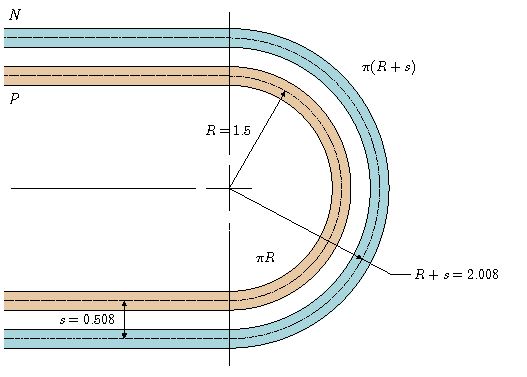
\includegraphics[width=\columnwidth]{fig_bend}
\caption{The 180-degree bend of fixture B, dimensions in mm. Centrelines are dash-dotted, and P is the inner trace. The
arc lengths $\pi R$ and $\pi(R + s)$ differ by $\pi s$ whatever the radius.}
\label{fig:bend}
\end{figure}

\begin{figure}[t]
\centering
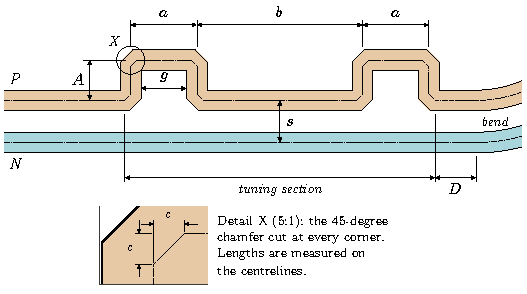
\includegraphics[width=\columnwidth]{fig_excursion}
\caption{One tuning section (C, $N = 2$) and the symbols used for it: amplitude $A$ between centrelines, top $a$
and gap $b$ along them, fold edge spacing $g$, pitch $s$, distance to the bend $D$. Every corner carries a
45-degree chamfer of leg $c$ (detail X, \DetailScale:1).}
\label{fig:excursion}
\end{figure}

\textbf{The fixture.} One microstrip layer over a return plane (Fig.~\ref{fig:xsec}, Table~\ref{tab:params}):
$h = 0.2$\,mm, $\varepsilon_r = 4.3$, $w = 0.25$\,mm, $s = 0.508$\,mm. Every bent variant uses the same U-bend
($R = 1.5$\,mm for P), the same 12\,mm legs and the same launch plane, so only the tuning differs
(Fig.~\ref{fig:families}):
A, a straight pair of the U-bend's mean length; B, the untuned bend; C, two sparse excursions next to the bend;
C far, the same two excursions next to the launch; D, a dense accordion of four; F, one broad trombone; and E, a
pair-level raised-cosine excursion of both traces together, a control whose net turning angle is zero and which
therefore leaves the length difference unchanged. Each single-trace tuning is cut into P on the leg leading into
the bend and turns away from N. Every route length change is intentional and listed in
Table~\ref{tab:metrics}. Clearance between P and N copper is checked by our generator and by KiCad~10's DRC
(\texttt{kicad-cli pcb drc}, 0.15\,mm rule), and no variant has a clearance or short violation. KiCad does not
check spacing within one net, so the fold spacing is set by the parameters, \FoldD\,mm edge to edge in D.

\begin{figure*}[t]
\centering
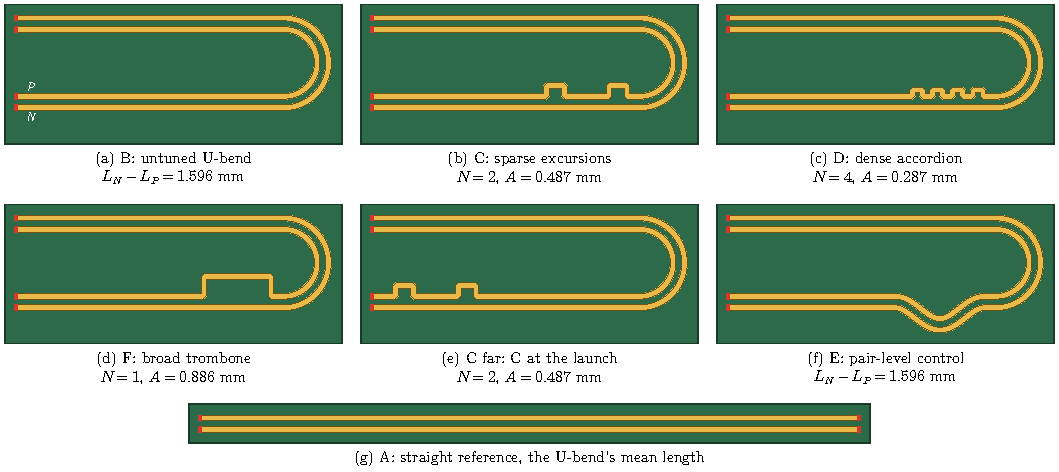
\includegraphics[width=\textwidth]{fig_variants}
\caption{The variants as openEMS is given them, all at one scale: the copper polygons (gold) and the four
50\,$\Omega$ lumped ports (red) on the substrate. In every tuned variant (b--e) P and N are exactly equal in
centreline length; $N$ is the number of excursions and $A$ the solved amplitude. A (g) is straight, as long as
the U-bend's mean centreline.}
\label{fig:families}
\end{figure*}

\begin{table}[t]
\centering
\caption{Parameters. All values are \textbf{proposed} for this study. None is calibrated to a laminate or a fabricator.}
\label{tab:params}
\scriptsize
\adjustbox{max width=\columnwidth}{\begin{tabular}{@{}llll@{}}\toprule
Parameter & Unit & Value & Range or note \\\midrule
Dielectric height $h$ & mm & 0.2 & fixed \\
Relative permittivity $\varepsilon_r$ & -- & 4.3 & fixed \\
Loss tangent at 5 GHz & -- & 0.02 & fixed, $\propto 1/f$ \\
Copper thickness / $\sigma$ & mm / MS/m & 0.035 / 58 & sheet model \\
Trace width $w$ & mm & 0.25 & fixed \\
Pair pitch $s$ (centre to centre) & mm & 0.508 & fixed, 20 mil \\
Bend radius of P, $R$ & mm & 1.5 & 0.75, 1.5, 3.0 \\
Leg length (launch to bend) & mm & 12.0 & fixed \\
Excursions $N$ & -- & 1, 2, 4 & F, C, D \\
Amplitude $A$ & mm & solved & 0.29--1.08 \\
Excursion top / gap & mm & 0.45--3.0 & per family \\
Corner chamfer & mm & 0.075 & fixed \\
Stripline plane spacing & mm & 0.7 & trace midway \\
Distance to bend $D$ & mm & 0.5 & 0.5 or at launch \\
Serpentine added length & mm & 6.0 & fold gap 1.0, 0.15 \\
Edge (10--90\,\%) & ps & 35--300 & post-processing \\
Bandwidth & GHz & 0--30 & Gaussian pulse \\
Finest cell (coarse/medium/fine) & \textmu m & 60/40/27 & convergence \\
\bottomrule\end{tabular}
}
\end{table}

\begin{figure}[t]
\centering
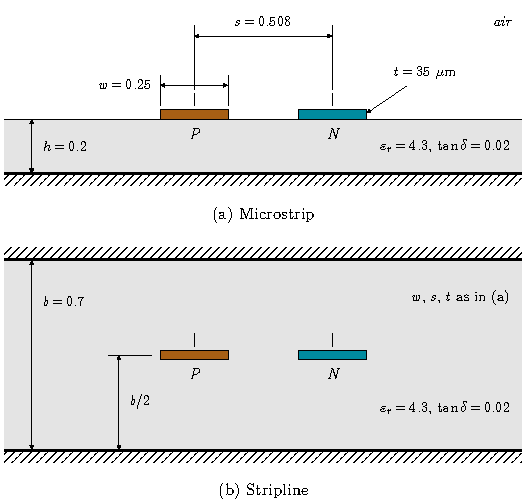
\includegraphics[width=\columnwidth]{fig_xsec}
\caption{Cross-sections at true scale, dimensions in mm. The stripline variants are the same copper midway
between two planes.}
\label{fig:xsec}
\end{figure}

\begin{figure*}[t]
\centering
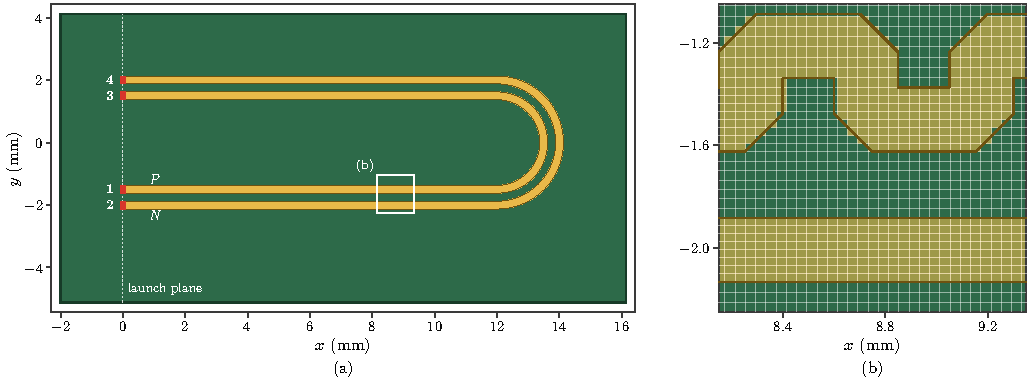
\includegraphics[width=\textwidth]{fig_model}
\caption{(a) Fixture B in its computational domain: the substrate extends 2\,mm past the copper on every side,
and the ports, numbered in mixed-mode order, sit on the launch plane. (b) The medium mesh
(\MediumCellUm\,$\mu$m finest cell) over D's first excursions. Cells whose centre lies in the copper are
filled, so the 45-degree chamfers are staircased.}
\label{fig:ports}
\end{figure*}

\begin{figure}[t]
\centering
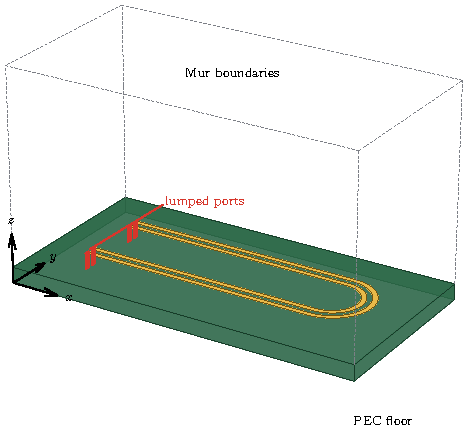
\includegraphics[width=\columnwidth]{fig_model3d}
\caption{The model of fixture B in three dimensions, height drawn \ModelZE{} times its true scale: the dielectric
slab on the PEC floor, the copper sheets, the lumped ports from the floor to the copper, and the edges of the
air box, whose five open faces are Mur boundaries.}
\label{fig:model3d}
\end{figure}

\begin{figure*}[t]
\centering
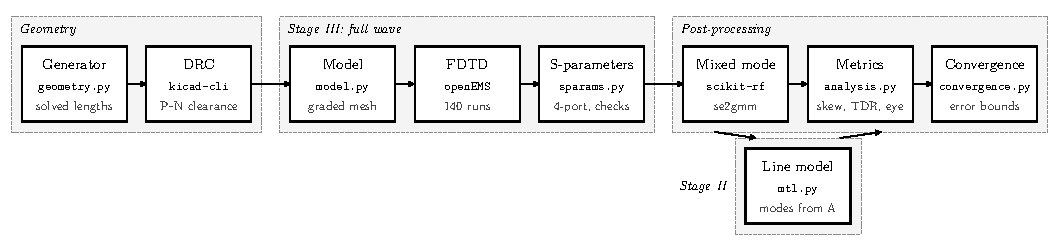
\includegraphics[width=\textwidth]{fig_flow}
\caption{The pipeline. The line model (Stage II) is calibrated on fixture A's mixed-mode parameters and read
beside the full-wave results. Each run keeps its model, its solver log and a provenance record (solver version, model hash, wall time, timesteps). Each variant keeps its \texttt{.s4p} and its checks.}
\label{fig:pipeline}
\end{figure*}

\section{Numerical model}
\label{sec:model}

\subsection{Stage II: a two-conductor line model}

For the pair, the coupled telegrapher equations are
\begin{equation}
  \frac{\mathrm{d}\mathbf{V}}{\mathrm{d}x} = -(\mathbf{R} + j\omega\mathbf{L})\,\mathbf{I}, \qquad
  \frac{\mathrm{d}\mathbf{I}}{\mathrm{d}x} = -(\mathbf{G} + j\omega\mathbf{C})\,\mathbf{V},
  \label{eq:telegrapher}
\end{equation}
with $2\times2$ per-unit-length matrices whose off-diagonal terms are the coupling~\cite{paul_mtl}. For a
symmetric pair the even and odd modes diagonalise them. We calibrate the modes on the full-wave straight fixture A rather than assume a cross-section. Its $\Sdd{}$ (100\,$\Omega$) and $\Scc{}$ (25\,$\Omega$) are each the
two-port of a uniform line, and the extraction of Eisenstadt and Eo~\cite{eisenstadt1992} gives
$Z_\mathrm{odd} = \ZOdd\,\Omega$ ($Z_\mathrm{diff} = \ZDiff\,\Omega$), $Z_\mathrm{even} = \ZEven\,\Omega$
($Z_\mathrm{comm} = \ZComm\,\Omega$), $\eeff = \EpsOdd$ (odd) and \EpsEven{} (even), with loss and dispersion over
the whole band (the values quoted are means from 0.5 to 10\,GHz). Each variant is then a cascade of chain matrices, coupled where the traces run
together and uncoupled single lines (Hammerstad--Jensen parameters) where P leaves N or where N's excess lies in
the bend, spread over 18 slices. The model carries every length and none of the rest. Corners, coupling between
a meander's folds or across the U, and the bend as a discontinuity are all missing from it, so where it disagrees
with full wave the cause is something other than length.

\subsection{Stage III: full-wave extraction}

The solver is openEMS~\cite{openems_intro,liebig2013}, an equivalent-circuit FDTD code, version
\texttt{\SolverVersion}. Its Python bindings were not installed on the host, so the model is written directly in
the XML vocabulary those bindings produce, which we had checked against this openEMS version before. The
signal copper is a conducting sheet (35\,$\mu$m, 58\,MS/m) drawn from the generator's polygons. The return plane is
the PEC floor of the domain and the dielectric is a lossy box (Table~\ref{tab:params}). openEMS models the
loss as a fixed conductivity, so $\tan\delta$ falls as $1/f$. The other five faces are first-order Mur absorbing
boundaries~\cite{mur1981}, at least 2\,mm (10$h$) from any copper laterally and 2.5\,mm above it
(Fig.~\ref{fig:model3d}).

Each trace end has a 50\,$\Omega$ lumped port from the plane to the copper, on the launch plane $x = 0$
(Fig.~\ref{fig:ports}). Ports are numbered in scikit-rf's mixed-mode order~\cite{skrf_se2gmm}: 1 = P near,
2 = N near, 3 = P far, 4 = N far. Each variant takes four runs, each exciting one port with the other three
passive~\cite{openems_ports}, with a Gaussian pulse covering 0 to 30\,GHz. From each port's voltage $u_k$ and
current $i_k$ (into the structure), the power waves~\cite{kurokawa1965}
$a_k = (u_k + Z_0 i_k)/(2\sqrt{Z_0})$ and $b_k = (u_k - Z_0 i_k)/(2\sqrt{Z_0})$ give $S_{kj} = b_k/a_j$. The
result is written as a Touchstone \texttt{.s4p} from DC to 30\,GHz in 10\,MHz steps.

The mesh is rectilinear and graded. Its finest cells lie over the copper regions: 60, 40 and 27\,$\mu$m for the
coarse, medium and fine levels, with every straight trace edge on a grid line. Away from the copper the cells grow
by at most 1.3 per cell, to 0.15\,mm laterally and 0.3\,mm in the air. These limits are the same at every level, so
only the copper regions are refined. All bent variants share one mesh per level, built over the union of
their copper, so discretisation error in the copper they share is common to them. The medium mesh of the bent
fixtures has \CellsMedium\,M cells and the fine one \CellsFine\,M. The arcs and chamfers are staircased
(Fig.~\ref{fig:ports}b).

The pulse's DC content leaves a static field in the domain whose energy settles near $-38$\,dB, so no run
reaches an energy end criterion. A pulse without DC content does reach one, but it measures nothing useful below
about 2\,GHz. Every run therefore stops at a fixed 2\,ns of simulated time, by which the port voltages have
fallen at least \TruncWorst\,dB below their peak (Table~\ref{tab:checks}). On fixture B (coarse mesh, port 1
excited) a 7\,ns record changes the low-frequency S-parameters by about $10^{-3}$.

\section{Analysis metrics}
\label{sec:metrics}

\textbf{Mixed mode.} \texttt{se2gmm(p=2)} on the order above gives $d_\mathrm{near}, d_\mathrm{far},
c_\mathrm{near}, c_\mathrm{far}$, so $\Sdd{11}=S_{00}$, $\Sdd{21}=S_{10}$, $\Scd{21}=S_{30}$ (zero-based), with
reference impedances of 100\,$\Omega$ differential and 25\,$\Omega$ common, in scikit-rf~\cite{arsenovic2022}. We
checked this convention against the scikit-rf 2.2.0 source rather than its rendered documentation.

\textbf{Waveforms.} A differential step of 1\,V open circuit (+1\,V and $-1$\,V, each behind 50\,$\Omega$) with a
Gaussian edge of 10--90\,\% rise time $t_r$ drives ports 1 and 2, and ports 3 and 4 are 50\,$\Omega$ to the plane
(100\,$\Omega$ differential, 25\,$\Omega$ common). Far-end voltages follow by superposition from the four-port in
the frequency domain and an inverse FFT, with nothing fitted. $V_d = V_P - V_N$, $V_c = (V_P + V_N)/2$.

\textbf{Skew} is $t_{50}(N\ \text{falling}) - t_{50}(P\ \text{rising})$ at the far end, each at half its own final
value. Positive means P, the inner trace, arrives first. We report 50\,ps edges unless stated, and 35 to 300\,ps
in Section~\ref{sec:results}. Edges faster than 35\,ps are not evaluated, because the simulated band ends at
30\,GHz.

\textbf{Delay efficiency.}
\begin{equation}
  \eta = \frac{t_\mathrm{skew,ref} - t_\mathrm{skew}}{\Delta L_\mathrm{add}\sqrt{\eeff^\mathrm{single}}/c},
  \label{eq:eta}
\end{equation}
where the reference is the identical untuned fixture (B, or the straight serpentine reference), $\Delta
L_\mathrm{add}$ is the centreline the tuning adds to P, and $\eeff^\mathrm{single} = \EpsSingle$
(\PsPerMm\,ps/mm) is the velocity a designer's length-to-delay conversion would use. $\eta = 1$ means the delay
is what the length predicts. On the same basis the untuned bend has $\eta = \BendEta$.

\textbf{Other metrics}, each over 0.1--20\,GHz unless stated: worst $|\Sdd{11}|$; RMS $|\Scd{21}|$; differential
TDR impedance from the step response of $\Sdd{11}$ with a 35\,ps edge; the frequency-resolved skew of
Eq.~\eqref{eq:fdskew}; a PRBS7 eye at 10\,Gb/s (50\,ps edges) and 16\,Gb/s (35\,ps edges), with height at the
best phase and width where the eye is open by more than 10\,\% of the swing; and the board area of the tuning,
its length times its amplitude. No interface specification is assumed, so wherever a pass or fail would need one the
target is illustrative and is to be selected for the intended interface.

\begin{table*}[t]
\centering
\caption{Metrics, medium mesh, 50\,ps edge. $\Delta L_\mathrm{add}$ is the centreline the tuning adds to P;
$\eta$ is Eq.~\eqref{eq:eta}; MTL is the line model's skew; $|\Sdd{11}|$ and $|\Scd{21}|$ over 0.1--20\,GHz;
$Z_\mathrm{diff}$ from TDR. Skew bounds: each variant's own where it was solved on three or more meshes; $^\dagger$~borrowed from the
converged variant whose smallest features it shares, not a convergence result for this variant
(Section~\ref{sec:verification}).}
\label{tab:metrics}
\footnotesize
\adjustbox{max width=\textwidth}{% metric table
\begin{tabular}{@{}lrrrrrrrrr@{}}\toprule
Variant & $\Delta L_\mathrm{add}$ & Skew & $\eta$ & MTL & $V_c$ p-p & $|S_{dd11}|$ & $|S_{cd21}|$ & $Z_\mathrm{diff}$ & Area \\
 & (mm) & (ps) & & (ps) & (\%) & max (dB) & RMS (dB) & max ($\Omega$) & (mm$^2$) \\\midrule
A straight & -- & 0.00 $\pm$ 0.05 & -- & 0.00 & 0.00 & -23.4 & -- & 106.0 & 0.00 \\
B untuned & -- & 9.27 $\pm$ 0.05 & -- & 8.83 & 4.87 & -20.7 & -10.2 & 107.1 & 0.00 \\
E pair exc. & -- & 9.39 $\pm$ 0.05 & -- & 8.83 & 4.92 & -21.4 & -10.1 & 108.1 & 4.00 \\
C sparse & 1.596 & 3.59 $\pm$ 0.31 & 0.60 & 0.31 & 1.83 & -21.6 & -18.0 & 106.9 & 1.83 \\
C far & 1.596 & 4.36 $\pm$ 0.31 & 0.52 & 0.96 & 2.19 & -19.6 & -15.4 & 106.9 & 1.83 \\
D dense & 1.596 & 5.16 $\pm$ 0.43 & 0.44 & 0.27 & 2.67 & -19.8 & -14.9 & 106.9 & 0.95 \\
F trombone & 1.596 & 2.29 $\pm$ 0.31 & 0.74 & 0.23 & 1.16 & -16.8 & -22.0 & 114.4 & 2.79 \\
C, EM-sized & 2.213 & 0.56 $\pm$ 0.31 & 0.66 & -2.98 & 0.52 & -21.7 & -25.2 & 106.7 & 2.40 \\
D, EM-sized & 2.484 & 1.90 $\pm$ 0.43 & 0.50 & -4.50 & 0.98 & -19.9 & -22.6 & 106.7 & 1.31 \\
F, EM-sized & 1.991 & 0.15 $\pm$ 0.31 & 0.77 & -1.89 & 0.40 & -16.7 & -27.8 & 115.0 & 3.41 \\
\bottomrule\end{tabular}
}
\end{table*}

\begin{figure*}[t]
\centering
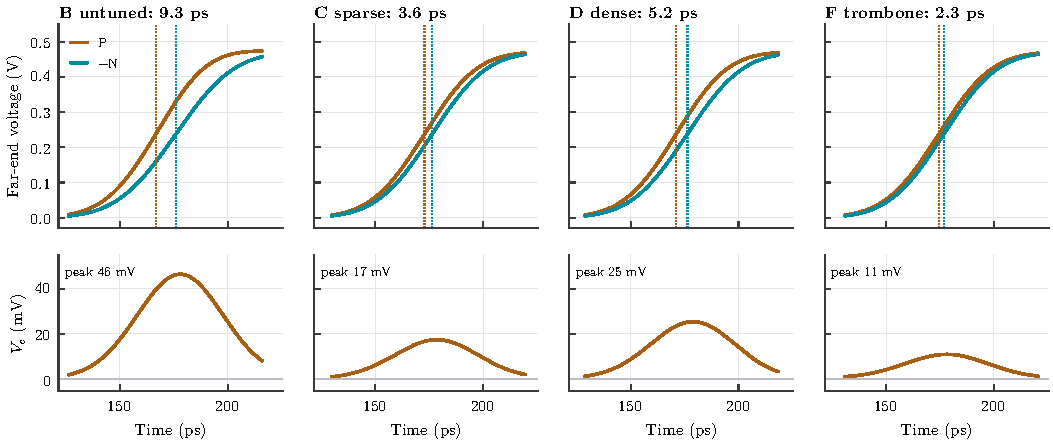
\includegraphics[width=\textwidth]{fig_waveforms}
\caption{Far-end P and $-$N for a differential step (50\,ps edge), and the common-mode voltage. Dotted lines mark
each 50\,\% crossing.}
\label{fig:waveforms}
\end{figure*}

\section{Verification of the numerics}
\label{sec:verification}

Table~\ref{tab:checks} lists the checks for every variant. Reciprocity holds to $|S_{ij}-S_{ji}| \le$
\RecipMax{} (the straight fixture, symmetric by construction, to \RecipA). Every four-port is passive, with a
largest singular value of $S$ over the band of \PassB{} for B and no more than \PassMax{} for any variant. Every
record ends with its port voltages at least \TruncWorst\,dB below their peak.

\textbf{Convergence.} B, C, D and the serpentine set were solved on three meshes and D on a fourth
(Table~\ref{tab:conv}, Fig.~\ref{fig:conv}). We report Roache's grid convergence index~\cite{roache1994}
over the three finest meshes, with safety factor 1.25 and an observed order capped at the scheme's formal order
of 2. Where those meshes do not converge monotonically we use three times their spread. B converges monotonically, with a formal GCI of \GciB\,ps on the finest mesh. D's 75\,$\mu$m chamfers span barely one cell
on the coarse mesh, and its coarse value is the outlier. Over the three finest meshes it converges monotonically,
to \ExtD\,ps. The tight serpentine's 0.15\,mm folds still oscillate across meshes. Two caveats apply to every
bound. The outer cell limits are the same at every level, so only the copper regions are refined. And where the
meshes do converge monotonically the observed order is \OrderB{} for B and \OrderD{} for D, well above the
scheme's formal order of 2. The three levels are therefore not in the asymptotic range. That is why the order is capped, and why the
finest-mesh GCIs are formal values rather than demonstrated ones. One cause is that only the
straight legs have their copper edges on mesh lines. The tops and verticals of the tuning sections do not, so each level
sees an amplitude and a vertical's width quantized to its own cell, by up to half a cell. The comparison tables quote the
medium mesh throughout, so each medium value carries its own bound, 1.25 times its distance from the extrapolated
value, or three times the spread where the meshes oscillate (Table~\ref{tab:conv}). That gives $\pm$\BoundMedB\,ps for B,
$\pm$\BoundMedC\,ps for C and $\pm$\BoundMedD\,ps for D, whose medium value runs high by about that much. A
variant solved on the medium mesh only carries the bound of the converged variant whose smallest features it
shares: C's for C far, F and the EM-sized C and F; D's for the EM-sized D; B's for E and the other bend radii.
These borrowed bounds are not convergence results for those variants. Table~\ref{tab:metrics} marks them with
$^\dagger$, and Fig.~\ref{fig:skew} draws them dashed.
Because a wide bound can hide a
trend or invent one, we also judge every conclusion mesh by mesh. Table~\ref{tab:etalevels} gives $\eta$ on each mesh, against the
untuned reference on the same mesh.

\begin{table}[t]
\centering
\caption{Numerical checks (medium mesh). Truncation is how far every port voltage had fallen, relative to its
peak, over the last 5\,\% of the record.}
\label{tab:checks}
\scriptsize
\adjustbox{max width=\columnwidth}{\begin{tabular}{@{}lrrr@{}}\toprule
Variant & Reciprocity & Passivity & Truncation \\
 & $\max|S_{ij}-S_{ji}|$ & $\max\sigma(S)$ & (dB) \\\midrule
A straight & $3.3\times10^{-7}$ & 0.989 & -110 \\
B untuned & $2.4\times10^{-3}$ & 0.989 & -110 \\
C sparse & $4.5\times10^{-3}$ & 0.988 & -110 \\
C far & $2.8\times10^{-3}$ & 0.988 & -109 \\
D dense & $3.4\times10^{-3}$ & 0.988 & -110 \\
E pair exc. & $2.9\times10^{-3}$ & 0.988 & -110 \\
F trombone & $2.8\times10^{-3}$ & 0.988 & -110 \\
C, EM-sized & $3.7\times10^{-3}$ & 0.988 & -110 \\
D, EM-sized & $3.0\times10^{-3}$ & 0.988 & -110 \\
F, EM-sized & $2.0\times10^{-3}$ & 0.988 & -110 \\
Serp. ref. & $6.0\times10^{-5}$ & 0.989 & -110 \\
Serp. 1.0 mm & $1.8\times10^{-3}$ & 0.988 & -109 \\
Serp. 0.15 mm & $2.1\times10^{-3}$ & 0.988 & -109 \\
B, R 0.75 & $3.5\times10^{-3}$ & 0.990 & -110 \\
B, R 3.0 & $2.4\times10^{-3}$ & 0.987 & -108 \\
B stripline & $1.8\times10^{-3}$ & 0.989 & -109 \\
C stripline & $1.4\times10^{-3}$ & 0.988 & -109 \\
D stripline & $1.8\times10^{-3}$ & 0.988 & -110 \\
F stripline & $2.2\times10^{-3}$ & 0.988 & -109 \\
Serp. ref. SL & $2.9\times10^{-5}$ & 0.988 & -99 \\
Serp. 1.0 mm SL & $1.5\times10^{-3}$ & 0.987 & -98 \\
Serp. 0.15 mm SL & $1.5\times10^{-3}$ & 0.987 & -98 \\
\bottomrule\end{tabular}
}
\end{table}

\begin{table}[t]
\centering
\caption{Mesh convergence of the skew (50\,ps edge). The finest-mesh GCI is the formal value. The 40\,\textmu m bound is what the comparison tables carry (Section~\ref{sec:verification}).}
\label{tab:conv}
\scriptsize
\adjustbox{max width=\columnwidth}{\begin{tabular}{@{}lrrrrrrl@{}}\toprule
Variant & 60\,\textmu m & 40\,\textmu m & 27\,\textmu m & 18\,\textmu m & GCI & 40\,\textmu m & Convergence \\
 & (ps) & (ps) & (ps) & (ps) & finest & bound & \\\midrule
B untuned & 9.54 & 9.27 & 9.25 & -- & $\pm$0.02 & $\pm$0.05 & monotonic \\
C sparse & 3.69 & 3.59 & 3.61 & -- & $\pm$0.31 & $\pm$0.31 & oscillatory \\
D dense & 4.45 & 5.16 & 4.88 & 4.84 & $\pm$0.03 & $\pm$0.43 & monotonic \\
Serp. ref. & 0.03 & 0.03 & 0.03 & -- & $\pm$0.00 & $\pm$0.00 & monotonic \\
Serp. 1.0 mm & -32.41 & -29.99 & -29.69 & -- & $\pm$0.31 & $\pm$0.68 & monotonic \\
Serp. 0.15 mm & -23.63 & -24.12 & -22.98 & -- & $\pm$3.40 & $\pm$3.40 & oscillatory \\
\bottomrule\end{tabular}
}
\end{table}

\begin{table}[t]
\centering
\caption{Delay efficiency $\eta$ (Eq.~\ref{eq:eta}) on each mesh, against the untuned reference on the same
mesh. D at 18\,\textmu m has no B at that level and is compared with B at 27\,\textmu m.}
\label{tab:etalevels}
\scriptsize
\adjustbox{max width=\columnwidth}{\begin{tabular}{@{}lrrrr@{}}\toprule
$\eta$ on each mesh & 60\,\textmu m & 40\,\textmu m & 27\,\textmu m & 18\,\textmu m \\\midrule
C sparse & 0.62 & 0.60 & 0.60 & -- \\
D dense & 0.54 & 0.44 & 0.46 & 0.47 \\
Serp. 1.0 mm & 0.91 & 0.84 & 0.84 & -- \\
Serp. 0.15 mm & 0.67 & 0.68 & 0.65 & -- \\
\bottomrule\end{tabular}
}
\end{table}

\begin{figure}[t]
\centering
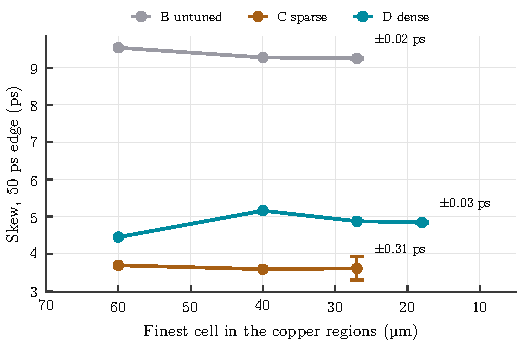
\includegraphics[width=\columnwidth]{fig_convergence}
\caption{Skew against the finest cell size. The bar on each variant's finest point is its formal GCI bound (Section~\ref{sec:verification}).}
\label{fig:conv}
\end{figure}

\section{Results}
\label{sec:results}

All values in this section are simulated. Table~\ref{tab:metrics} collects them.

\subsection{The untuned bend}

B shows \SkewB\,ps of skew at 50\,ps edges, against \SkewSingle\,ps from Eq.~\eqref{eq:dt} with the single-line
$\eeff$, so geometry predicts the bend to \BendErrPct\,\% by this metric. The line model, which holds the same
lengths and the two modal velocities and nothing else, reads \MtlB\,ps by the same metric. Part of what a
50\,\% crossing makes of a pure length difference in a coupled pair is the mode conversion that difference
causes, so the agreement with Eq.~\eqref{eq:dt} is specific to the metric. The skew does depend on the edge,
\SkewBRdf\,ps at 35\,ps and
\SkewBRdaa\,ps at 300\,ps (Fig.~\ref{fig:rise}), moving from near the odd-mode prediction (\SkewOdd\,ps) toward
the even-mode one (\SkewEven\,ps) as the edge slows. The bend radius matters a little where Eq.~\eqref{eq:dl} says
it should not, with \SkewBRsmall\,ps at $R = 0.75$\,mm, \SkewB\,ps at 1.5\,mm and \SkewBRlarge\,ps at 3\,mm
(Fig.~\ref{fig:radius}). The pair-level excursion E leaves the skew where B has it (\SkewE\,ps) and adds
\DelayAddE\,ps of pair delay, as designed.

\subsection{Equal length is not equal delay}

Fig.~\ref{fig:skew} is the central result. Every single-trace tuning makes P and N equal in centreline length, and every one leaves skew. The broad trombone
F leaves \SkewF\,ps and the two sparse excursions C leave \SkewC\,ps, both $\pm$\UncC\,ps (C's own bound, borrowed for
F). The dense accordion D leaves \SkewD\,ps ($\pm$\UncD\,ps), and \ExtD\,ps extrapolated over its meshes. In efficiency terms
(Eq.~\eqref{eq:eta}), $\eta = \EtaF$, \EtaC{} and \EtaD{} for one, two and four excursions. The transmission-line
model, given the same lengths, predicts \MtlF, \MtlC{} and \MtlD\,ps. The waveforms (Fig.~\ref{fig:waveforms})
show the same thing at the receiver. P still leads N, and the common-mode pulse falls from
\(\VcB\)\,\% of the step for B to \VcF--\VcD\,\%, not to zero.

\begin{figure}[t]
\centering
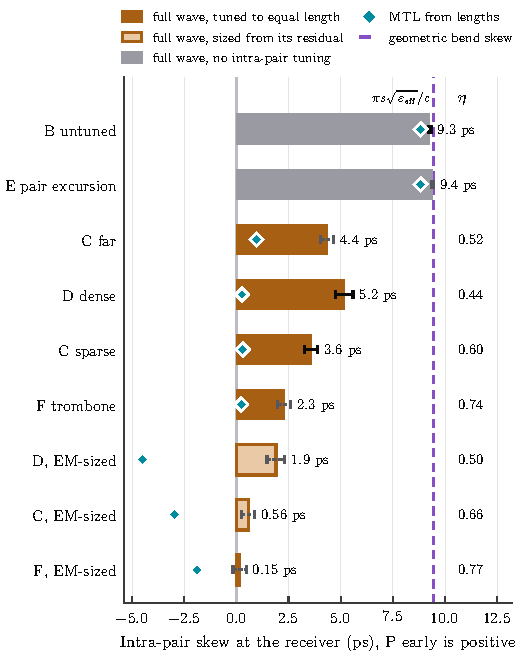
\includegraphics[width=\columnwidth]{fig_skew}
\caption{Skew at the receiver, 50\,ps edge. Copper: tuned to exactly equal length. Grey: no intra-pair tuning.
Diamonds: the transmission-line model with the same lengths. Bars: mesh-based bounds, solid where the variant was
solved on three or more meshes, dashed where the bound is borrowed from a converged variant.}
\label{fig:skew}
\end{figure}

\begin{figure*}[t]
\centering
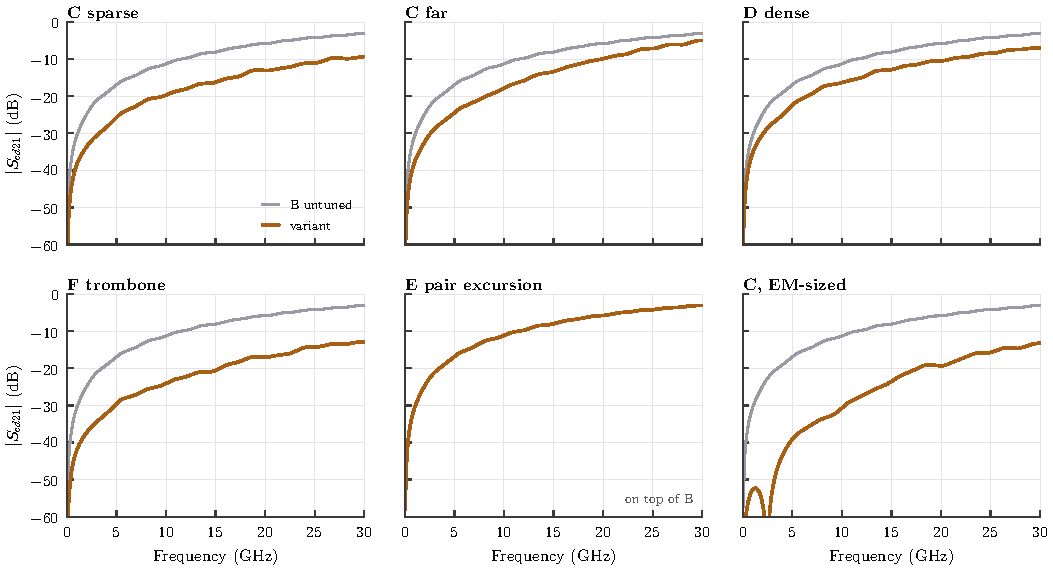
\includegraphics[width=\textwidth]{fig_scd21}
\caption{$|\Scd{21}|$ of each variant (copper) against the untuned bend B (grey).}
\label{fig:scd21}
\end{figure*}

\subsection{Where the delay goes}

The gap is consistent with two effects that the line model leaves out, coupling between the folds of a meander
and its corners. The serpentine experiment varies the first. It is a straight pair with 6\,mm added to P in three
excursions, once with folds 1.0\,mm apart (5$h$) and once 0.15\,mm apart, the clearance rule. The two have the same corners, the same amplitude and the same added length. Their section lengths differ,
\SecLenSloose{} against \SecLenStight\,mm, so P also runs uncoupled from N over a different length. With loose folds
$\eta = \EtaSloose$ (\EtaMinSloose--\EtaMaxSloose{} across the meshes). With tight folds it is \EtaStight{}
(\EtaMinStight--\EtaMaxStight), \FoldPenMin{} to \FoldPenMax{} points lower on every mesh
(Fig.~\ref{fig:eta}, Table~\ref{tab:etalevels}). The difference is consistent with coupling between the folds,
but this pair of runs does not exclude the change in uncoupled length. The loose serpentine's own shortfall,
which the line model also misses, is consistent with an effect of its twelve corners. No run here varies the
corners alone, so that attribution is by elimination. We define the shortfall per excursion of a bend correction as the skew the line model says the tuning removed less
the skew full wave says it removed, net of the \MtlBendErr\,ps the model misses on the bare bend. It is \PerExcF,
\PerExcC{} and \PerExcD\,ps for F, C and D. It is not a constant. It falls as the excursions get
smaller and more numerous, but more slowly than their number grows, so the total shortfall still rises from one
excursion to four. The three families change the excursion count, the amplitude and the fold spacing together,
so this experiment does not separate them. The serpentines separate fold spacing alone, and the EM-sized
variants of Section~\ref{sec:optimization} test the amplitude. The dense accordion D has the most corners and
the closest folds, and the lowest $\eta$.

\begin{figure}[t]
\centering
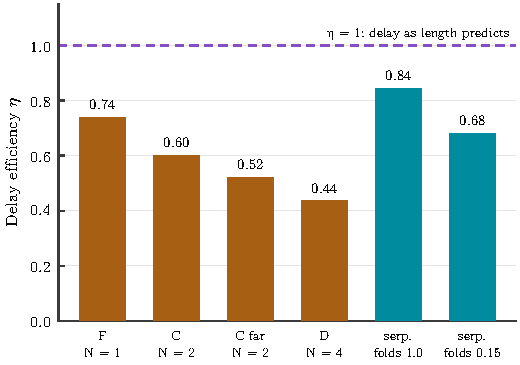
\includegraphics[width=\columnwidth]{fig_eta}
\caption{Delay efficiency $\eta$ (Eq.~\ref{eq:eta}) of the bend corrections (copper, $N$ excursions) and of the
6\,mm serpentines (teal) with loose and tight folds.}
\label{fig:eta}
\end{figure}

\begin{figure*}[t]
\centering
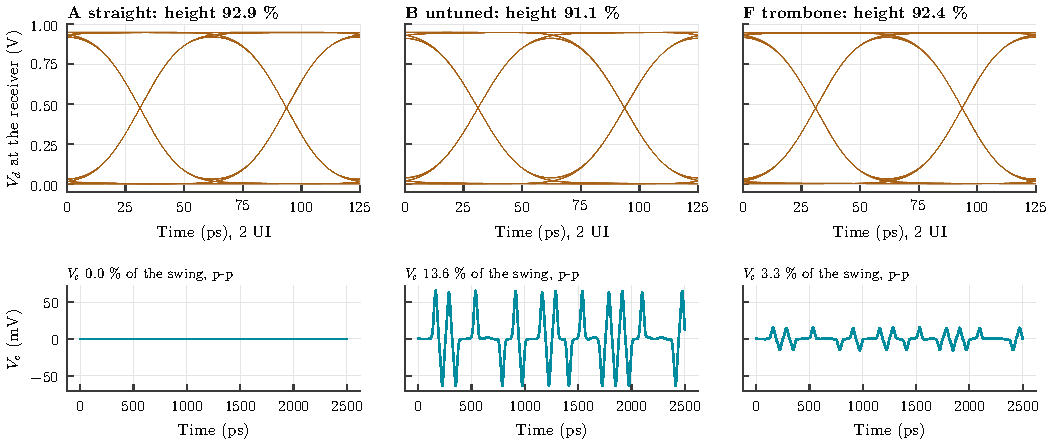
\includegraphics[width=\textwidth]{fig_eye}
\caption{16\,Gb/s PRBS7 eyes (35\,ps edges) and the common-mode voltage at the receiver.}
\label{fig:eye}
\end{figure*}

\subsection{Stripline}

The results above are all microstrip, where the odd and even modes travel at different velocities. We solved B, C, D, F and the serpentine set again in stripline to see whether that matters. The copper is the
same, midway between two planes 0.7\,mm apart, with the ports to the lower plane. Stripline is homogeneous, so its nominal velocity is
$c/\sqrt{\varepsilon_r}$ (\PsPerMmSl\,ps/mm) and Eq.~\eqref{eq:eta} uses that. Geometry predicts the bend to
\BendErrPctSl\,\% (\SkewBsl\,ps against \SkewGeoSl\,ps). The length-matched tunings remove \RemovedPctFsl,
\RemovedPctCsl{} and \RemovedPctDsl\,\% of it for F, C and D, against \RemovedPctF, \RemovedPctC{} and
\RemovedPctD\,\% in microstrip, and the serpentines give $\eta = \EtaSloosesl$ and \EtaStightsl, a fold
penalty of \FoldPenaltySl{} points against \FoldPenalty{} in microstrip (Fig.~\ref{fig:stripline}). We had
expected less, since in a homogeneous medium the far-end coupling between parallel lines vanishes. One possible explanation, not tested here, is that the folds of a meander carry current in opposite directions.
What couples them would then act backward along the route, and backward coupling is present in both media. These stripline runs are on the medium mesh only.

\begin{figure}[t]
\centering
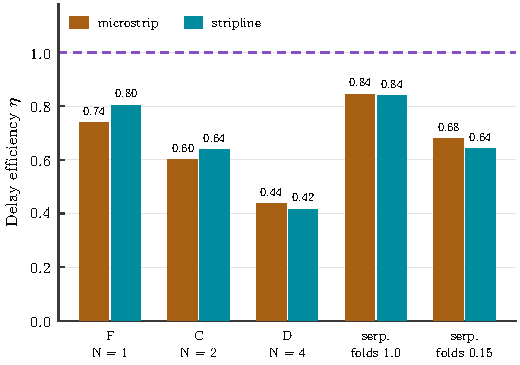
\includegraphics[width=\columnwidth]{fig_stripline}
\caption{Delay efficiency of the same copper in microstrip and in stripline, each against its own nominal
velocity.}
\label{fig:stripline}
\end{figure}

\subsection{Placement}

C far is the same tuning as C, next to the launch instead of the bend. Its arrival skew is close
(\SkewCfar{} against \SkewC\,ps), but its mode conversion is not. Between the tuning and the bend the pair
carries a skew in the other direction, and the two conversions drift apart in phase with frequency. The
frequency-resolved skew of C far climbs from \FdCfarGf\,ps at 5\,GHz to \FdCfarGcf\,ps at 25\,GHz, while C stays
near \FdCGf\,ps (Fig.~\ref{fig:fdskew}). Its peak $|\Scd{21}|$ to 20\,GHz is \ScdMaxCfar\,dB against
\ScdMaxC\,dB for C. In this one comparison, compensation next to the mismatch did better. Two placements are not
a sweep of the distance.

\begin{figure}[t]
\centering
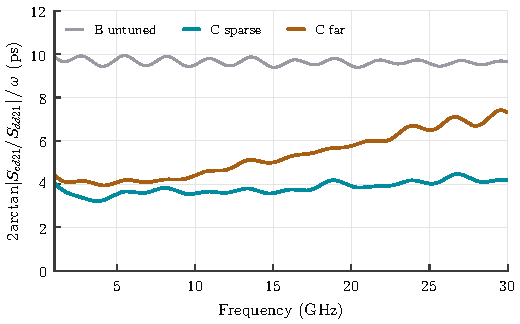
\includegraphics[width=\columnwidth]{fig_fd_skew}
\caption{Frequency-resolved skew from Eq.~\eqref{eq:fdskew}. Compensation far from the bend (C far) holds at low
frequency and fails as frequency rises.}
\label{fig:fdskew}
\end{figure}

\subsection[Reflection, impedance and mode conversion]{Reflection, impedance and\protect\\ mode conversion}

Where a trace leaves its partner, the differential impedance rises. The broad trombone F, whose P moves \AmpF\,mm further from N for 3\,mm, lifts $Z_\mathrm{diff}$ to \ZmaxF\,$\Omega$ against \ZmaxB\,$\Omega$ for the untuned bend
(Fig.~\ref{fig:tdr}), and has the worst return loss of the set (\SddMaxF\,dB against \SddMaxB\,dB,
Fig.~\ref{fig:sdd}), so the variant with the least residual skew pays for it in reflection. The dense accordion
barely moves $Z_\mathrm{diff}$. Mode conversion follows the residual skew: across the nine bend variants, RMS $|\Scd{21}|$ falls in the same
order as the skew (Fig.~\ref{fig:scd21}, Table~\ref{tab:metrics}), and E's curve lies on top of B's.

\begin{figure}[t]
\centering
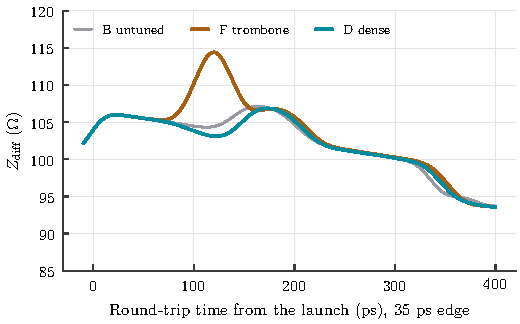
\includegraphics[width=\columnwidth]{fig_tdr}
\caption{Differential TDR (35\,ps edge). F's uncoupled stretch shows as the peak near 120\,ps.}
\label{fig:tdr}
\end{figure}

\begin{figure}[t]
\centering
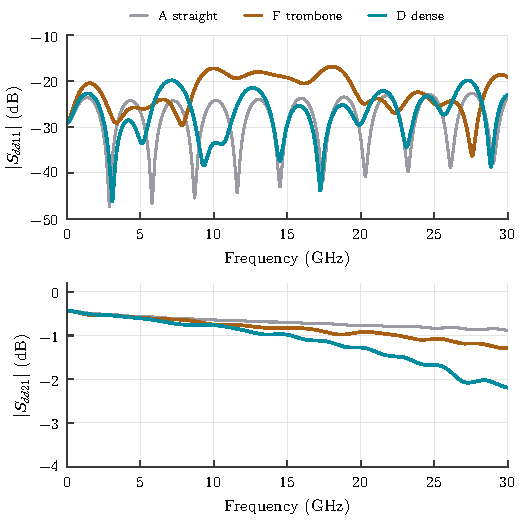
\includegraphics[width=\columnwidth]{fig_sdd}
\caption{Differential return and insertion loss of the straight reference A, the trombone F and the dense
accordion D.}
\label{fig:sdd}
\end{figure}

\begin{figure}[t]
\centering
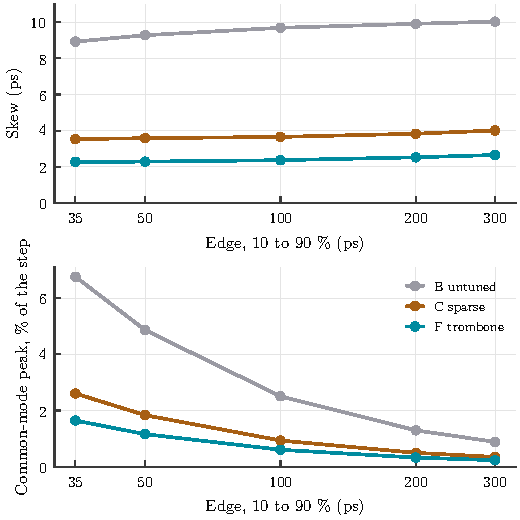
\includegraphics[width=\columnwidth]{fig_rise}
\caption{Skew and peak common-mode voltage against the edge rate.}
\label{fig:rise}
\end{figure}

\subsection{What the skew does to a signal}

At 16\,Gb/s with 35\,ps edges, the untuned bend closes the differential eye from \EyeHA\,\% to \EyeHB\,\% of the
swing and leaves its width at \EyeWB\,UI (Fig.~\ref{fig:eye}). The larger effect is common mode, \EyeVcB\,\% of
the swing peak to peak at the receiver against \EyeVcF\,\% for F. For a receiver with good common-mode rejection
the skew of a single bend is a common-mode problem more than a timing one. Whether that common mode radiates
depends on the structure beyond the pair, which this study does not model.

\begin{figure}[t]
\centering
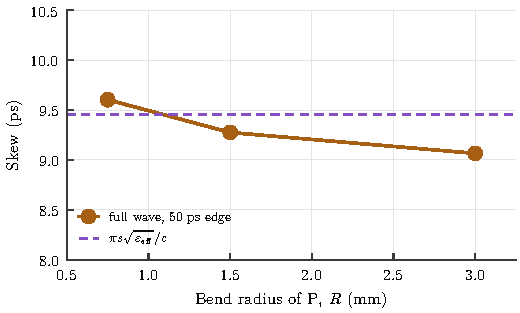
\includegraphics[width=\columnwidth]{fig_radius}
\caption{Skew of the untuned bend against its radius.}
\label{fig:radius}
\end{figure}

\section{EM-informed sizing}
\label{sec:optimization}

\textbf{One correction step.} This is not an optimizer. It takes the residual of one field solution, corrects the amplitude once and solves again. It was not
iterated. If each excursion loses a fixed amount of delay to its corners and folds, more
amplitude on the same excursions should recover it. We lengthened C, D and F by their own medium-mesh residual,
converted to length at the bend's rate ($\Delta L_\mathrm{add} = \pi s\,(1 + t_\mathrm{skew}/t_\mathrm{skew,B})$).
By CAD measure P is now longer than N, with \AddedCcal, \AddedDcal{} and \AddedFcal\,mm added in total. By length
alone these variants now overshoot. The line model, which holds only lengths, predicts \MtlFcal,
\MtlCcal{} and \MtlDcal\,ps. Full wave gives \SkewFcal\,ps for F and \SkewCcal\,ps for C, within the bound borrowed from C, though neither variant
was solved on more than one mesh. D comes down only to \SkewDcal\,ps. It was sized from its medium-mesh residual, which
Section~\ref{sec:verification} puts about \BoundMedD\,ps high, so if anything it was over-corrected. This tests the
fixed-shortfall model. The model holds for the trombone, roughly for the sparse tuning and not for the
accordion. The extra millimetres delivered
\MargPctF\,\% of their expected delay in F and \MargPctC\,\% in C, but only \MargPctD\,\% in D. That is consistent with its lengthened verticals coupling more strongly to one
another, which no run here isolates. A broad or sparse tuning is calibrated by one field
solution or one set of coupons per stackup, and a tuner could carry the per-excursion correction. A dense
accordion needs iteration, which is one more reason to avoid it.

\textbf{Pareto comparison.} Over the bent candidates we minimise four objectives defined above, $|t_\mathrm{skew}|$
(50\,ps edge), RMS $|\Scd{21}|$, worst $|\Sdd{11}|$ and tuning area, with no weighted score. The
non-dominated set is \{\ParetoAll\}. B is on it only because the untuned bend has no tuning area. E adds area and removes nothing, so B dominates
it. Fig.~\ref{fig:pareto} shows two projections. Against area the dense
accordion is cheap and weak, and against return loss the trombone trades reflection for skew.

\begin{figure*}[t]
\centering
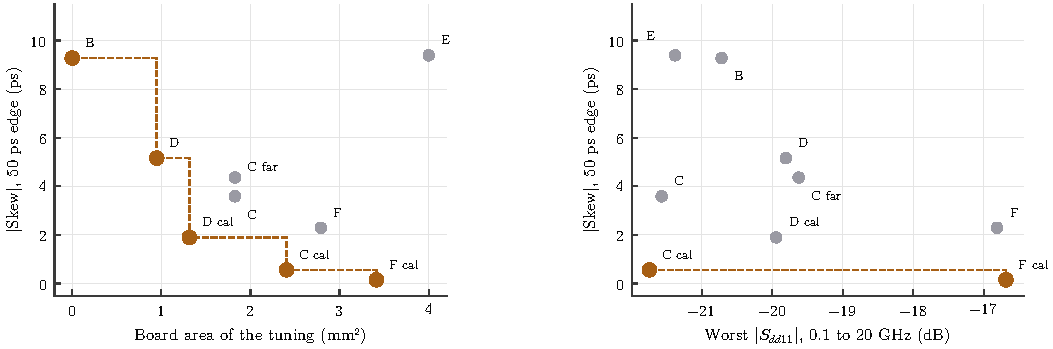
\includegraphics[width=\textwidth]{fig_pareto}
\caption{Two projections of the four-objective comparison. Copper points are non-dominated in that projection, and the dashed line joins them.}
\label{fig:pareto}
\end{figure*}

\section{Physical validation plan}
\label{sec:validation}

This plan has not been executed. It calls for a coupon panel with one coupon per variant (A--F, the EM-sized variants and the serpentines), each in
three copies, on one laminate and stackup. All coupons share one launch design, either edge-mount connectors or GSSG
probe pads with ground vias. A 2x-thru of the launch alone on the same panel allows fixture de-embedding as in IEEE
Std~370~\cite{ieee370}. Measure four-port S-parameters to 30\,GHz on a calibrated VNA and de-embed them to the
launch plane. Microsection one coupon per panel to measure $w$, $s$, $h$ and the copper. Extract $\eeff$ of the odd
and even modes from coupon A and rerun the EM with the measured dimensions before comparing. The comparison covers skew, $\eta$ (Eq.~\ref{eq:eta}, against B on the same panel), $|\Sdd{11}|$, $|\Scd{21}|$
and TDR. Error bars combine the spread of the three copies, the VNA's stated uncertainty and the GCI here. Three predictions are to be tested. Equal-length tuning should leave \SkewF{} to \SkewD\,ps at this pitch, the
shortfall should grow with the excursion count and the same should hold on a stripline panel.
Near- or far-field scanning would be needed only if emission is the claim, which it is not here.

\section{Recommendations}
\label{sec:recommendations}

For edge-coupled pairs at this pitch and coupling, in microstrip and stripline and with the caveat that the
numbers are simulated:
\begin{itemize}\itemsep 1pt
\item Expect geometry to predict a bend's skew well (here within \BendErrPct\,\% at a 50\,ps edge, and
\SkewBRdaa\,ps at 300\,ps), and expect it to over-predict what a
length-matched tuning removes. Budget a residual, or size the tuning from a field solution or a coupon.
\item Prefer few excursions. The shortfall per excursion shrinks with its size, but not as fast as the count
grows. A single excursion removed \RemovedPctF\,\% of the skew, four removed \RemovedPctD\,\%.
\item Keep folds apart. Here folds at the clearance rule lost \FoldPenMin--\FoldPenMax{} points of efficiency
against folds
5$h$ apart.
\item Tune next to the mismatch. The same correction at the launch matches arrival time but not phase at high
frequency.
\item Watch the impedance of a broad excursion. The uncoupled stretch lifts $Z_\mathrm{diff}$, here to
\ZmaxF\,$\Omega$. Keep its amplitude small relative to the pitch or keep it short.
\item A pair-level excursion does not fix intra-pair skew.
\item The stripline check, on one mesh, showed the same pattern. The bend's skew matched geometry to
\BendErrPctSl\,\%, the length-matched tunings removed a similar share, and tight folds cost \FoldPenaltySl{} points. The edge rate and the interface decide whether a few
picoseconds matter. At 16\,Gb/s here they matter more as common mode than as eye closure.
\end{itemize}

\section{Reproducibility}
\label{sec:repro}

The study's repository, to be published with the report, holds \texttt{parameters.yaml}; \texttt{scripts/} with the geometry generator (and its KiCad
export and DRC), the openEMS model writer, the run orchestrator with provenance, the S-parameter extraction, the
line model, the analysis, the convergence study and the figure and table generators; and \texttt{figures/}. Every
number in this report is a macro generated from \texttt{build/results/results.json}. We made the \RunCount{} runs on one
Linux host, \RunHours\,h of wall time in all on single-threaded solver processes. The
\texttt{README.md} lists the commands, and regenerating every figure and table from the stored S-parameters takes a
few minutes.

\section{Limitations}
\label{sec:limitations}

One width and one pitch, in one microstrip and one stripline stackup. The stripline ports run to the lower
plane only, and its plane spacing came from a closed-form estimate. Its $Z_\mathrm{diff}$ is about
\ZmaxBsl\,$\Omega$ by TDR, so its absolute return loss is worse than microstrip's, which does not affect the
skew comparisons. The return plane is a perfect conductor and the copper a
conducting sheet, so conductor loss is approximate and roughness is absent. The dielectric loss model has
$\tan\delta \propto 1/f$. Lumped ports at the launch are not a connector or a probe. We assume their reflection is common to every variant
and cancels in the comparisons. Because the variants' input impedances differ, the assumption may not hold exactly, and it was not tested. It does not
hold for absolute return loss. The staircased mesh resolves the
smallest features (the 75\,$\mu$m chamfers) with under two cells (\ChamferCellsMedium) at the medium level. The convergence study bounds the effect for B, C, D and the serpentines only. The stripline set was solved on
one mesh. Edges faster than 35\,ps and frequencies above 30\,GHz are outside the
simulated band. Common-mode voltage and $\Scd{21}$ are not emissions. Every full-wave result comes from one solver, openEMS. The line model is calibrated on its results, so their agreement is not independent validation. No second solver
was used. The mechanisms are not isolated: the corner effect is inferred by elimination, and the serpentine pair
varies fold spacing and uncoupled length together.

\section{Conclusions}

For this fixture at a 20\,mil pitch, the U-bend's skew was about 9\,ps, as geometry predicts. Matching the lengths
did not remove it. A length-matched serpentine removed between \RemovedPctD{} and \RemovedPctF\,\% of the skew in full-wave
simulation, and the
remainder grew with the number of excursions and the closeness of the folds. A line model with the same lengths
missed nearly all of it, and the same copper in stripline behaved the same way. One field-solver iteration sized
the broad and sparse tunings to within \SkewFcal{} and \SkewCcal\,ps, and the dense accordion needed more. In these simulations more length matching did
not close the gap. Size the tuning by what it does electrically, and keep it next to the bend with few excursions set
well apart.
